\section{Software Design}
\subsection{Architecture}
We have chosen to do some initial architectural modeling, even though we follow the SCRUM development methodology, which initially does not have an architectural modeling phase. This is because the system that are being developed, could easily end up becoming larger and more complex than initially thought. \\ 
The goal of the initial achitectural modeling is not to write tons of documentation and end up with a final plan, but rather to identify and agree on an architectural and technical  strategy within the development team. The architectural model will be more complex and detailed later during development. \\
By performing some high-level architectural modeling at the beginning of the project, we hope to improve alot of other factors throughout the project. \cite{agilemodeling}

\begin{itemize}
	\item This will allow us to think about some of the more critical issues we will be facing, and potentially avoid spending time on something that woud prove later to be impossible, because of this we will most likely get \textbf{improved productivity}
	\item The project will be at a \textbf{reduced technical risk} bacuse the team would have some sort of vision on how to solve problems before encountering them. 
	\item \textbf{Development time} will also hopefully be reduced, given that better decisions and estimates could be taken.
	\item The high-level architecture models will \textbf{improve communication} within the team because it helps with sharing thoughts on how to solve problems.
	\item This will also \textbf{improve team organization} because it will make it easier to delegate tasks between each SCRUM sprint.
\end{itemize}

Bacuse of our development method we have to be careful not to spend too much time on the initial achitectural modeling. The amount of value we get from doing the modeling drasticly drops if we oversaturate the model.\\
Figure 4. shows a graphical representation of the value of initial architectural modeling over time.
\begin{figure}[H]
\fbox{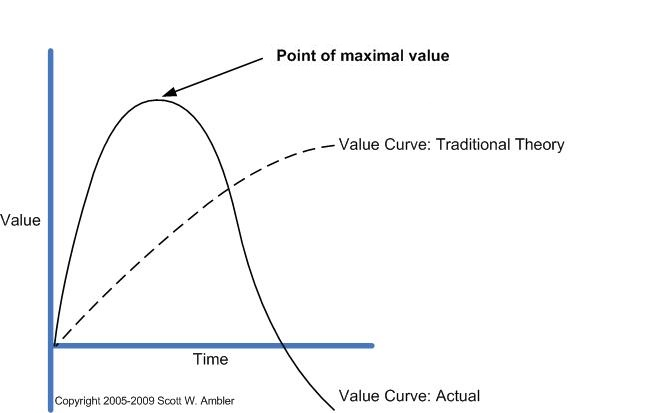
\includegraphics[scale=0.8]{graphics/valueOfModeling}}
\caption{Value of modeling \cite{valueofmodeling}}
\end{figure}

Since we are not locked to a certain method of doing architectural modeling, we have chosen to only model a user interface flow chart, a UML deployment diagram and a technology stack diagram. We believe these models will help the team the most without spending too much time modeling.

% Client-Server backend: REST Web-services for compatibility with default EmberJS API 
% Model-View-Whatever frontend: EmberJS presents data with views determined by controllers through user interaction (i.e clicking a link sends the "action" (what link was clicked) for processing by the controller, which loads data from the model and sends it to the appropriate view for rendering)